%=============================================================================
\section{Results}
\label{sec:results}
%=============================================================================

\subsection{RQ1: Does the Typed Representation Help?}
\label{sec:rq1}

Table~\ref{tab:rq1} and Fig.~\ref{fig:rq1} report pooled out-of-fold PR-AUC over all prefixes.
All learned detectors are far above the prevalence floor (0.054).
M1 reaches 0.479 [0.278, 0.759].
It is clearly better than the hand-weighted typology score B1 ($+0.268$, $p=0.010$) and than bag-of-actions B2 ($+0.363$, $p=0.003$), so the combination of temporal, structural and typed features matters far more than counting red flags or action types.
It is also above the GRU over typed tokens S1 (0.368), although that gap is not significant ($p=0.29$).

The comparison that isolates the representation is M1 against B3$'$, the same learner on flat features.
Over all prefixes B3$'$ is slightly higher (0.518), but the paired difference, $-0.038$ [$-0.139$, $+0.067]$, $p=0.68$, is small relative to its uncertainty.
The representation study in Fig.~\ref{fig:3c} shows the same picture: adding typed-action or motif groups to the flat set changes pooled PR-AUC by $-0.063$ and $-0.018$ (both $p>0.3$).
The mean of per-incident PR-AUC, which weights incidents equally instead of by their number of prefixes, ranks M1 first (0.708 vs.\ 0.628 for B3$'$).
Per incident (Fig.~\ref{fig:3b}) M1 is ahead on FEG (1.00 vs.\ 0.22, all nine actions are mixer deposits), WOOFi and BSC Token Hub, and behind on Paraluni, Ronin and DeltaPrime.
The per-incident gap does not correlate significantly with trajectory length (Spearman $\rho=-0.41$, $p=0.17$, $n=13$; HackerDAO and New Free DAO have no negatives with a complete cache and are excluded).
\textbf{Answer to RQ1:} over all prefixes, typing and motifs neither help nor hurt significantly at $N=15$; where they help is at the earliest prefixes (Sect.~\ref{sec:rq2}).

\begin{table}[t]
\centering
\caption{Detection quality under leave-one-incident-out evaluation (15 incidents, 1{,}384 pooled prefix rows, 8.4\% positive). Pooled PR-AUC with incident-bootstrap 95\% CI; mean of per-incident PR-AUC (13 incidents with negatives); paired difference to M1 with two-sided bootstrap $p$.}
\label{tab:rq1}
\small
\setlength{\tabcolsep}{4pt}
\resizebox{\linewidth}{!}{%
\begin{tabular}{@{}llccc@{}}
\toprule
ID & Detector & Pooled PR-AUC [95\% CI] & Mean/incident & M1 $-$ X ($p$) \\
\midrule
B0 & Prevalence & 0.054 [0.037, 0.097] & 0.142 & -- \\
B1 & Rule-based typology score & 0.212 [0.124, 0.410] & 0.460 & $+0.268$ (0.010) \\
B2 & Bag of actions + logistic reg. & 0.117 [0.068, 0.297] & 0.407 & $+0.363$ (0.003) \\
B3 & Flat features + random forest & 0.452 [0.277, 0.716] & 0.688 & $+0.028$ (0.60) \\
B3$'$ & Flat features + XGBoost (M1's learner) & 0.518 [0.319, 0.735] & 0.628 & $-0.038$ (0.68) \\
S1 & GRU over typed action tokens & 0.368 [0.221, 0.583] & 0.516 & $+0.111$ (0.29) \\
\textbf{M1} & \textbf{Flat + typed actions + motifs} & \textbf{0.479 [0.278, 0.759]} & \textbf{0.708} & -- \\
\midrule
 & Nested selection of bridge features & 0.490 [0.282, 0.753] & 0.650 & $-0.011$ (0.92) \\
\bottomrule
\end{tabular}}
\end{table}

\begin{figure}[t]
\centering
\begin{subfigure}[t]{0.49\linewidth}\centering
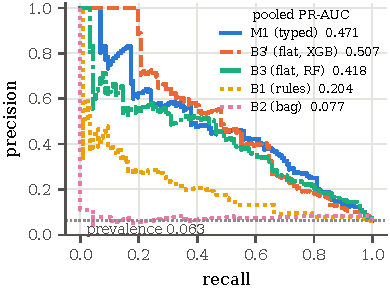
\includegraphics[width=\linewidth]{figures/fig3a.pdf}
\caption{Pooled PR curves.}
\label{fig:3a}
\end{subfigure}\hfill
\begin{subfigure}[t]{0.49\linewidth}\centering
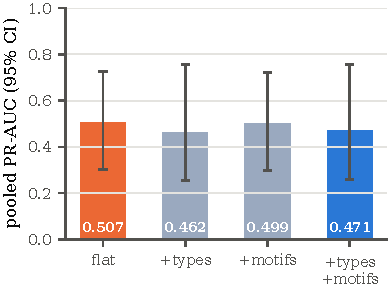
\includegraphics[width=\linewidth]{figures/fig3b.pdf}
\caption{Per-incident PR-AUC.}
\label{fig:3b}
\end{subfigure}\\[4pt]
\centering
\begin{subfigure}[t]{0.49\linewidth}\centering
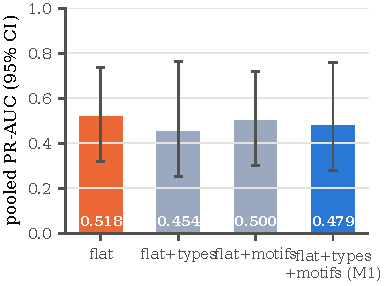
\includegraphics[width=\linewidth]{figures/fig3c.pdf}
\caption{Same learner, growing representation.}
\label{fig:3c}
\end{subfigure}
\caption{RQ1: detection over all prefixes. The learner is fixed in (c); only the feature groups change.}
\label{fig:rq1}
\end{figure}

\subsection{RQ2: How Early?}
\label{sec:rq2}

\paragraph{Online horizons.}
Figure~\ref{fig:4b} scores every trajectory at the prefix available $h$ minutes after its first action, which is what a live monitor sees.
One minute after the first action (median $k=2$ for incidents), M1 reaches PR-AUC 0.421 against 0.215 for B3$'$, a paired gain of $+0.206$ [0.032, 0.330], $p=0.010$.
The same holds at the absolute checkpoint $k=2$ (0.418 vs.\ 0.209, $+0.210$ [0.037, 0.333], $p=0.008$).
From five minutes on, the two representations are statistically indistinguishable, and B3$'$ is numerically ahead once flows are longer than about 15 actions, when amounts, fan-out and hop depth have had time to develop.
Both curves rise with the horizon, from about 0.4 in the first minute to 0.63--0.71 after one day.
Because we test eight horizons, the two significant early results would not survive a Bonferroni correction ($0.05/8=0.006$); we read them as consistent evidence, supported by both the online and the checkpoint view, that event types carry the signal when there is no structure yet.

\paragraph{Relative checkpoints.}
Figure~\ref{fig:4a} shows the retrospective view.
With a quarter of each trajectory observed M1 reaches 0.483 and with the complete trajectory 0.702 (B3$'$: 0.566 and 0.811); each checkpoint has 15 positive and 393 negative rows (3.7\% positive).
Figure~\ref{fig:4c} shows why early alerts are possible at all: the median calibrated score of incidents rises within the first 10\% of the trajectory and stays around 0.3--0.5, while the median negative stays near 0.03.

\begin{figure}[t]
\centering
\begin{subfigure}[t]{0.49\linewidth}\centering
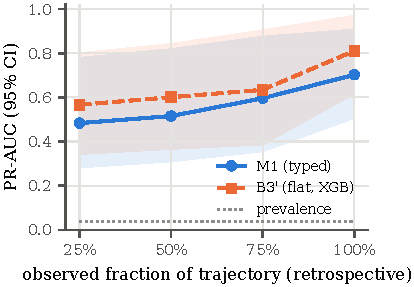
\includegraphics[width=\linewidth]{figures/fig4a.pdf}
\caption{Relative checkpoints.}
\label{fig:4a}
\end{subfigure}\hfill
\begin{subfigure}[t]{0.49\linewidth}\centering
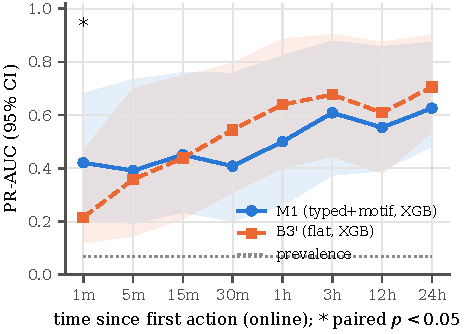
\includegraphics[width=\linewidth]{figures/fig4b.pdf}
\caption{Online horizons.}
\label{fig:4b}
\end{subfigure}\\[4pt]
\centering
\begin{subfigure}[t]{0.49\linewidth}\centering
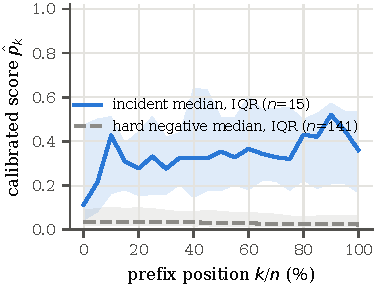
\includegraphics[width=\linewidth]{figures/fig4c.pdf}
\caption{Score along the trajectory.}
\label{fig:4c}
\end{subfigure}
\caption{RQ2: how early the signal appears. Shaded bands are incident-bootstrap 95\% CIs in (a,b) and interquartile ranges in (c).}
\label{fig:rq2}
\end{figure}

\paragraph{Alerts, lead time and false alerts.}
We replay every trajectory action by action, score each prefix $k\ge2$ with the calibrated M1 of its held-out fold, and record the first crossing of $\theta$ (Table~\ref{tab:lead}, Fig.~\ref{fig:rq2b}).
At $\theta=0.5$, 12 of 15 incidents raise an alert, and 12 of the 206 negatives that have at least two actions (5.8\%) raise a false alert; the other 187 negatives consist of a single action and are never scored.
Of the 10 incidents with a confirmed endpoint, three are alerted before the exit: DeltaPrime 114 minutes and six steps early, Chibi Finance 7.5 minutes and 17 steps early, and Radiant Capital 5 minutes and five steps early.
Four endpoints (FEG, New Free DAO, XKingdom, BSC Token Hub) are the \emph{first} action of the trace, the attacker sending the proceeds straight into a mixer, bridge or lending market, so no prefix-based detector can warn before them; of the six incidents where an early alert is possible, three receive one.
Raising $\theta$ trades detections for false alerts: at 0.7 the false-alert rate drops to 1.9\% but only one incident is alerted early.

\begin{table}[t]
\centering
\caption{RQ2: first alerts of calibrated M1 when every prefix $k\ge2$ is scored online. ``Before $t_e$'' counts the 10 incidents with a confirmed endpoint; 4 of them have their endpoint at $k=1$ and cannot be alerted early. False alerts are per trajectory over the 206 negatives with $\ge2$ actions.}
\label{tab:lead}
\small
\resizebox{\linewidth}{!}{%
\begin{tabular}{@{}lccccc@{}}
\toprule
$\theta$ & Before $t_e$ & Median lead [IQR] & Late / never & Incidents alerted & False-alert rate \\
\midrule
0.3 & 3/10 & 7.5 min [6.4, 60.5] & 6 / 1 & 14/15 & 12.6\% (26/206) \\
0.5 & 3/10 & 7.5 min [6.4, 60.5] & 5 / 2 & 12/15 & 5.8\% (12/206) \\
0.7 & 1/10 & 7.5 min & 2 / 7 & 5/15 & 1.9\% (4/206) \\
0.9 & 0/10 & -- & 0 / 10 & 0/15 & 0.0\% (0/206) \\
\bottomrule
\end{tabular}}
\end{table}

\begin{figure}[t]
\centering
\begin{subfigure}[t]{0.49\linewidth}\centering
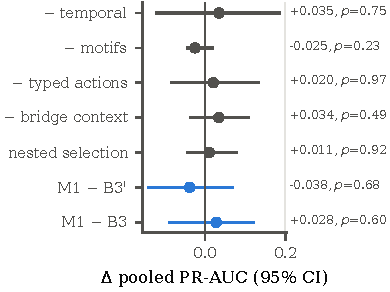
\includegraphics[width=\linewidth]{figures/fig5a.pdf}
\caption{Detection vs.\ false alerts.}
\label{fig:5a}
\end{subfigure}\hfill
\begin{subfigure}[t]{0.49\linewidth}\centering
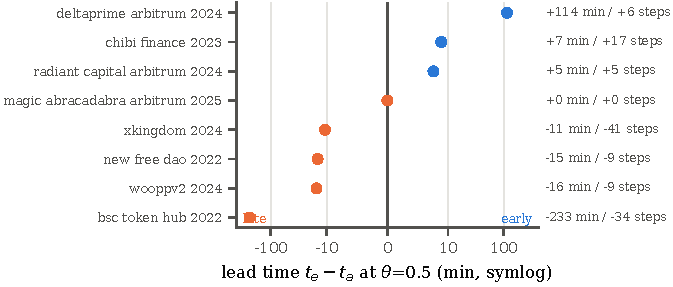
\includegraphics[width=\linewidth]{figures/fig5b.pdf}
\caption{Lead time per incident.}
\label{fig:5b}
\end{subfigure}\\[4pt]
\centering
\begin{subfigure}[t]{0.49\linewidth}\centering
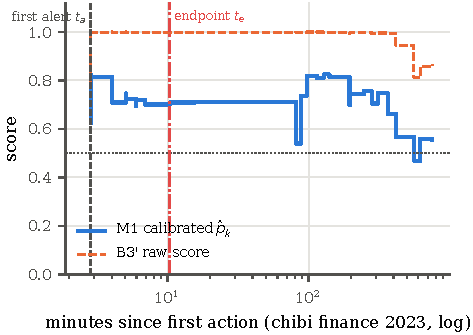
\includegraphics[width=\linewidth]{figures/fig5c.pdf}
\caption{Case study: Chibi Finance.}
\label{fig:5c}
\end{subfigure}
\caption{RQ2: alerting on the live replay. In (b) blue marks alerts before the endpoint and orange late alerts; incidents never alerted at $\theta=0.5$ are omitted.}
\label{fig:rq2b}
\end{figure}

\paragraph{Case study: Chibi Finance (2023).}
The exploiter of this Arbitrum rug pull made 40 actions in 12.6 hours; the endpoint is action 19, a Stargate bridge deposit 10 minutes after the first action (Fig.~\ref{fig:5c}).
After the second action, 2.8 minutes in, the calibrated score is 0.62 and the alert fires, 449\,s and 17 actions before the bridge deposit.
Its top TreeSHAP contributions are the mean log amount ($+1.50$), fan-out of the seed ($+0.84$) and a short mean gap between actions (170\,s, $+0.81$), followed by the absence of a bridge deposit so far ($+0.59$) and a swap share of 0.5 ($+0.53$): a large amount moving fast through a swap, i.e.\ AADAPT layering (ADT3028.003).
The score stays at or above 0.5 for 97\% of the remaining prefixes, through the bridge deposit and the following 12 hours.

\subsection{RQ3: Robustness, Calibration and Explanations}
\label{sec:rq3}

\paragraph{Ablations.}
Figure~\ref{fig:6a} removes one group at a time from M1.
No removal changes pooled PR-AUC significantly: temporal $+0.035$ ($p=0.75$), motifs $-0.025$ ($p=0.23$), typed actions $+0.020$ ($p=0.97$), bridge-context features $+0.034$ ($p=0.49$).
An earlier version of this pipeline dropped the bridge-context features after inspecting ablations on all incidents; choosing inside each training split instead (nested LOIO) keeps them in 3 of 15 folds and yields 0.490, within $0.011$ of M1 ($p=0.92$), so M1 as reported uses no post-hoc feature selection.

\paragraph{Calibration.}
Raw XGBoost scores are overconfident (ECE 0.071, Brier 0.075, Fig.~\ref{fig:6b}).
Platt scaling fitted on inner-fold scores reduces ECE to 0.015 [0.015, 0.071] and Brier to 0.062; isotonic regression reaches 0.021.
Calibrators are fitted per fold, so pooled PR-AUC over calibrated scores is lower (0.395) than over raw scores: calibration is used for thresholds and for the alert, not for ranking across folds.

\paragraph{Mimicry.}
We re-score each incident after inserting $j$ small decoy transfers to fresh addresses after every action (1\% of the value, one second apart), which dilutes type shares and motifs without changing the flow.
The fraction of incidents alerted within their first 400 actions falls from 80\% ($j=0$) to 60--67\% ($j\in\{1,2,4\}$), and the mean calibrated score at the 25\% checkpoint from 0.36 to 0.25 (Fig.~\ref{fig:6c}).
The detector degrades but is not blinded by cheap padding; an adaptive attacker who also slows down was not evaluated.

\paragraph{Builder settings.}
With one expansion round instead of two, trajectories are shorter (median 20 vs.\ 40 actions for incidents) and M1 is \emph{higher} (0.637--0.679 for $\eta\in\{5,10,20\}\%$) and above B3$'$ in all three settings (0.555--0.603).
With two rounds and $\eta\in\{10,20\}\%$, M1 is 0.554--0.566.
The ranking of M1 and B3$'$ thus depends on how far the trace is followed: deeper traces add long transfer chains in which amounts and hop depth dominate, while shallow traces keep the typed first steps in focus.

\begin{figure}[t]
\centering
\begin{subfigure}[t]{0.49\linewidth}\centering
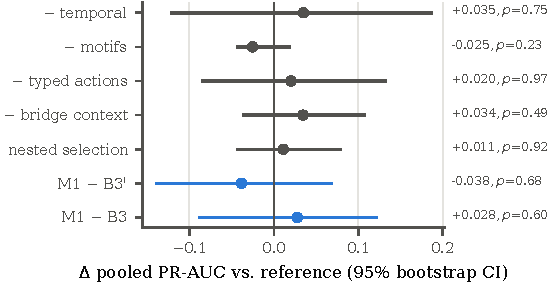
\includegraphics[width=\linewidth]{figures/fig6a.pdf}
\caption{Ablations (paired).}
\label{fig:6a}
\end{subfigure}\hfill
\begin{subfigure}[t]{0.49\linewidth}\centering
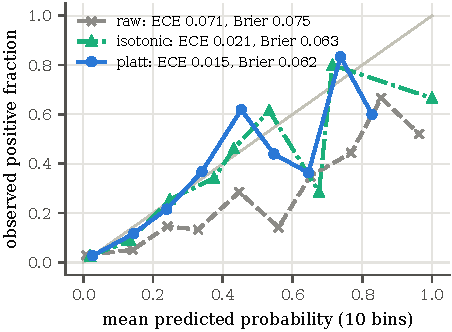
\includegraphics[width=\linewidth]{figures/fig6b.pdf}
\caption{Reliability diagram.}
\label{fig:6b}
\end{subfigure}\\[4pt]
\centering
\begin{subfigure}[t]{0.49\linewidth}\centering
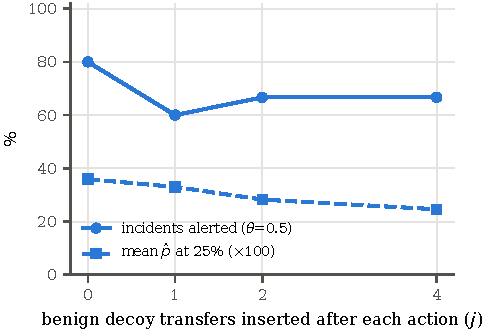
\includegraphics[width=\linewidth]{figures/fig6c.pdf}
\caption{Mimicry stress test.}
\label{fig:6c}
\end{subfigure}
\caption{RQ3: ablations, calibration and robustness to decoy transfers.}
\label{fig:rq3}
\end{figure}

\paragraph{What the model uses.}
Averaged over all prefixes (Fig.~\ref{fig:7a}), the largest TreeSHAP contributions come from the mean log amount, the bridge-deposit share, value retention, the mean gap between actions and the fan-out of the seed; typed features (bridge-deposit share, bigram diversity, transfer share, stablecoin legs) and the rapid-token-pivot motif make up five of the top twelve.
Stolen funds are large, move fast and leave the seed in few hops, whereas hard negatives are dominated by single bridge deposits of ordinary size (Fig.~\ref{fig:2b}).

\paragraph{Synthetic benchmark.}
On CAGI-Synth (Fig.~\ref{fig:7c}, synthetic data only), every learned detector reaches PR-AUC $\ge0.97$ at every difficulty, B1 stays below 0.18, and M1 trained on the real incidents and applied to synthetic data scores 0.014, below the synthetic prevalence (0.025).
Typology-based generators are thus \emph{easier} than real incidents and do not share their feature distribution; we release the generator as a sanity check and do not use synthetic results as evidence for any claim above.

\subsection{RQ4: Cost and Next-Action Forecasting}
\label{sec:rq4}

On a 4-core Intel Xeon at 2.1\,GHz, extracting the features of one prefix and scoring it takes a median of 11.7\,ms at $k=2$ and 23.6\,ms at $k=850$, with a peak memory increase below 0.2\,MB (Fig.~\ref{fig:7b}); re-scoring on every new action is far cheaper than the 12\,s Ethereum slot time, and end-to-end latency is dominated by the explorer API.
Before training a next-action model we fixed three data-sufficiency criteria: at least 1{,}000 transitions, at least 30 examples of each of the seven classes, and a majority class below 60\%.
The data pass the first (11{,}313 transitions) and fail the other two: transfers make up 67\% of transitions and lending deposits occur four times.
We therefore do not train a forecaster and report this as a negative result.

\begin{figure}[t]
\centering
\begin{subfigure}[t]{0.49\linewidth}\centering
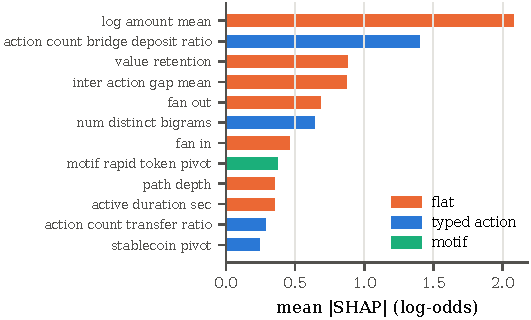
\includegraphics[width=\linewidth]{figures/fig7a.pdf}
\caption{Global TreeSHAP (top 12).}
\label{fig:7a}
\end{subfigure}\hfill
\begin{subfigure}[t]{0.49\linewidth}\centering
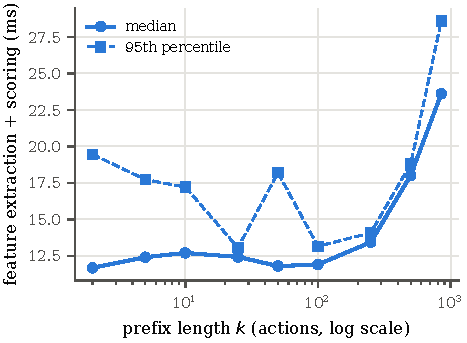
\includegraphics[width=\linewidth]{figures/fig7b.pdf}
\caption{Scoring latency on a CPU.}
\label{fig:7b}
\end{subfigure}\\[4pt]
\centering
\begin{subfigure}[t]{0.49\linewidth}\centering
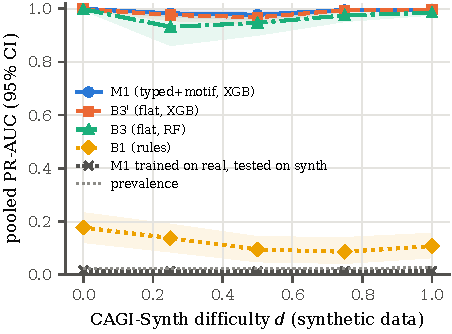
\includegraphics[width=\linewidth]{figures/fig7c.pdf}
\caption{CAGI-Synth (synthetic only).}
\label{fig:7c}
\end{subfigure}
\caption{What the model uses, what it costs, and the synthetic sanity benchmark.}
\label{fig:rq4}
\end{figure}
